\chapter{Двигатель постоянного тока}
\label{ch:chap1}
\newcommand\tab[1][1cm]{\hspace*{#1}}

\ExplSyntaxOn
\clist_new:N \l_feq_vector_clist
\NewDocumentCommand{\feqvector}{O{\\}mO{b}}{
  \clist_set:Nn \l_feq_vector_clist {#2} % Set the list
  \begin{#3matrix}
  \clist_use:Nn \l_feq_vector_clist {#1} % show it with separator from #1 (\\)
  \end{#3matrix}
}
\ExplSyntaxOff


Уравнения двигателя постоянного тока независимого возбуждения:
$$
  J\dot{\omega} = M, \tab M=k_mI, \tab I = \frac{U + \epsilon_i}{R}, \tab \epsilon_i = -k_e\omega
$$

В случае моего второго варианта уравнения примут конкретный вид:
$$
  0.0018\dot{\omega} = M, \tab M=0.3239I, \tab I = \frac{U + \epsilon_i}{4.6916}, \tab \epsilon_i = -0.3239\omega
$$

В нашем случае мы считаем напряжение $U(t)$ - входом объекта, а на выходе $\omega(t)$ - угловая скорость.

\section{Передаточная функция}
$$
\omega = \frac{\epsilon_i}{k_\epsilon} = -\frac{R}{k_\epsilon}I + \frac{1}{k_\epsilon}U = -\frac{R}{k_m k_\epsilon}M + \frac{1}{k_\epsilon}U = -\frac{RJ}{k_m k_\epsilon}p[\omega] + \frac{1}{k_\epsilon}U
$$ где $p[\omega]$ - дифференциальный оператор, производная от омеги
$$
\bigg(1 + \frac{RJ}{k_m k_\epsilon}p  \bigg)[\omega] = \frac{1}{k_\epsilon}U
$$
$$
\omega = \frac{k_m}{k_\epsilon k_m + RJp}[U]
$$
Перепишем через операторы лапласа, а также вынесем константу снизу за скобки для получения записи в инженерной форме, через постоянные времени $T$:
$$
\omega = \frac{k_m/k_mk_\epsilon}{\frac{RJ}{k_\epsilon k_m}s + 1}[U]
$$
Получим следующий общий вид апериодического звена первого порядка (тип звена):
$$
\omega = \frac{K}{Ts+1}[U]
$$, где $K = \frac{1}{k_\epsilon}$, $T = \frac{RJ}{k_\epsilon k_m}$

В моём случае константы двигателя будут выглядеть так:
$$
K \approx 3.08,\tab T \approx 0.08
$$

\section{Временные  характеристики}
Будем смотреть через \textbf{весовую} и \textbf{переходную} функции:

\begin{itemize}

\item Весовая функция - показывает реакцию системы на единичный импульс (в виде дельта-функции Дирака) при нулевых начальных условиях.
$$
y_{i.r.}(t) = \mathcal{L}^{-1}\{W(s)\}
$$
$$
y_{i.r.}(t) = \frac{1}{Tk_\epsilon}e^{-\frac{t}{T}}\theta(t)
$$, где $\theta(t)$ - функция Хевисайда. При наших коэффициентах:
$$
y_{i.r.}(t) = \frac{1}{0.259}e^{-\frac{t}{0.08}}\theta(t) \approx 38.5e^{-12.5t}\theta(t)
$$

\item Переходная функция - показывает реакцию системы на единичный скачок, "ступеньку", реализована при помощи функции Хевисайда, при нулевых начальных условиях.
$$
y_{s.r.} = \int y_{i.r.}(t) dt
$$
Но предпочтём вариант вычисления попроще\dots
$$
y_{s.r.} = \mathcal{L}^{-1}\{\frac{1}{s}W(s)\} = \frac{1}{k_\epsilon}(1-e^{-\frac{t}{T}})\textbf{1}(t) \approx \frac{1}{k_\epsilon}(1-e^{-\frac{t}{T}})\textbf{1}(t)
$$
где $\textbf{1}(t)$ - функция Хевисайда, но так как в симуляции единичный скачок происходит в $t=0$ момент времени, то его можно опустить. Аналогичное произойдёт и с дельта-функцией Дирака.
\end{itemize}


\begin{figure}[ht]
  \centering
  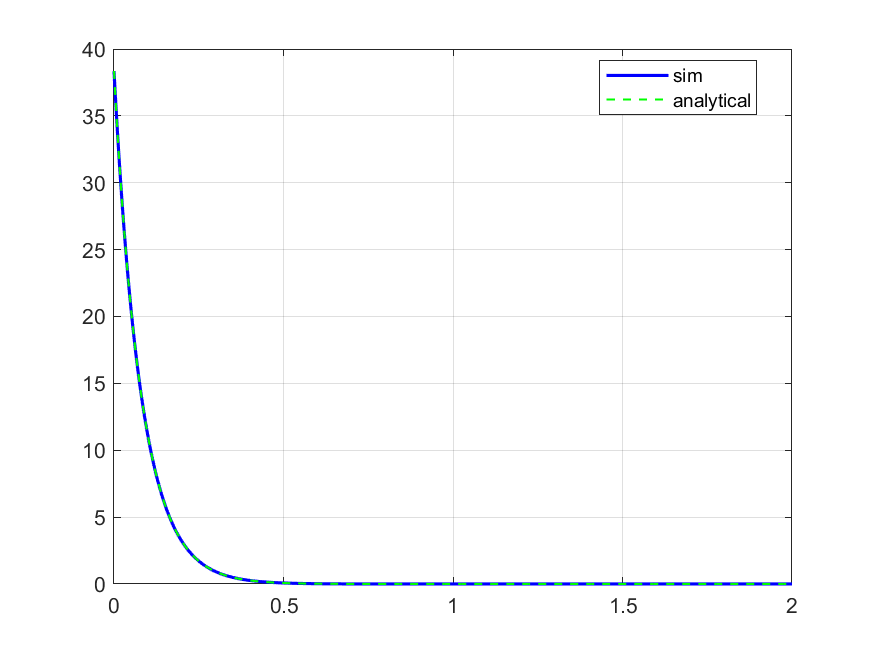
\includegraphics[width=0.8\textwidth]{impulse_responce1.png}
  \caption{Воздействие - \textrm{impulse responce}}
\end{figure}
\newpage
\begin{figure}[ht]
    \centering
    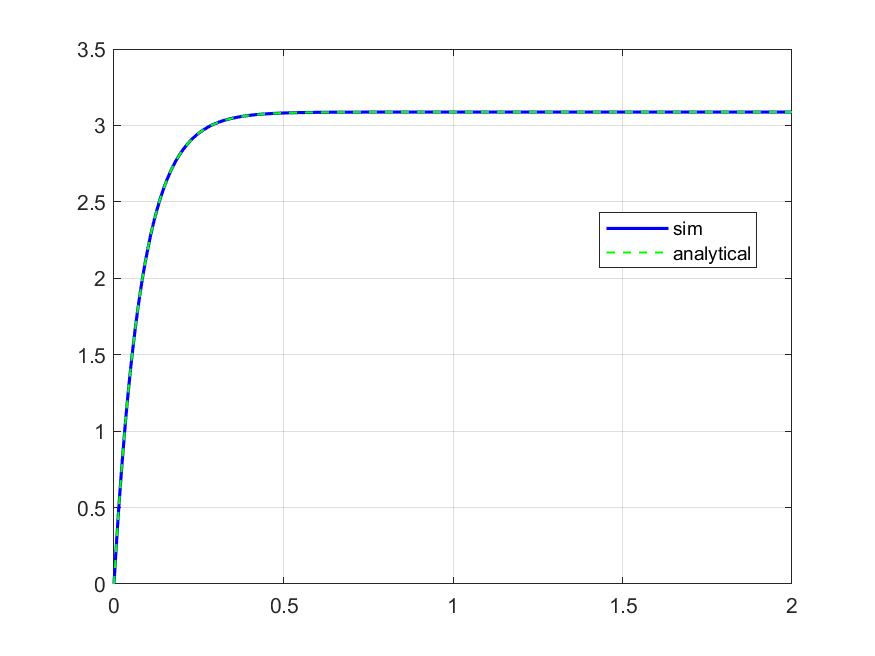
\includegraphics[width=0.8\textwidth]{step_responce1.png}
    \caption{Воздействие - \textrm{step responce}}
  \end{figure}
\newpage

\section{Частотные характеристики}

Запишем частотную-передаточную функцию, сделав простую замену: $s = j\omega$

$$
\begin{aligned}
  W(j\omega) = \frac{K}{jT\omega + 1} = \frac{K(jT\omega - 1)}{(jT\omega + 1)(jT\omega - 1)} = \\
    \frac{K(jT \omega - 1)}{ -\omega^2 T^2 - 1} = \frac{K}{ \omega^2 T^2 + 1} - j\frac{KT\omega }{ \omega^2 T^2 + 1} 
\end{aligned}
$$
Амплитудно-частотная характеристика:
$$
A(\omega) = \sqrt{P^2 + jQ^2} = \sqrt{\frac{K^2}{(\omega^2 T^2 + 1)^2} + \frac{K^2T^2\omega^2}{(\omega^2 T^2 + 1)^2} } = \frac{K}{\sqrt{1+T^2\omega^2}}
$$
Логарифмическая-Амплитудно-частотная характеристика:
$$
L(\omega) = 20lg(A) = 20lg(K) - 10lg(1+T^2\omega^2)
$$
Фазовая-частотная характеристика:
$$
\phi(\omega) = atan2(Q,P) = atan(-\omega T)
$$

\newpage
\begin{figure}[ht]
  \centering
  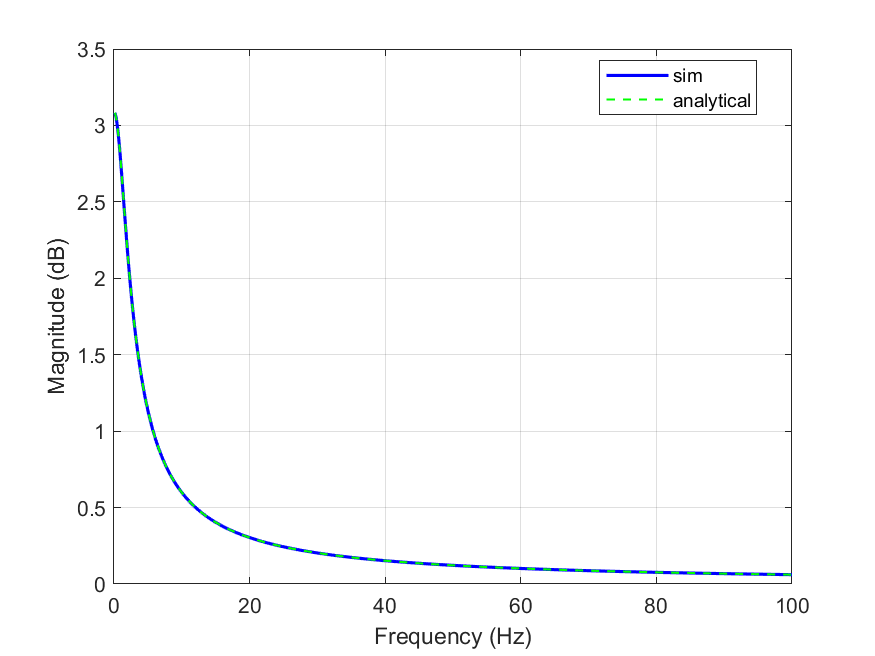
\includegraphics[width=0.8\textwidth]{freq_ampl1.png}
\caption{Сравнение - АЧХ}
\end{figure}

\begin{figure}[ht]
    \centering
    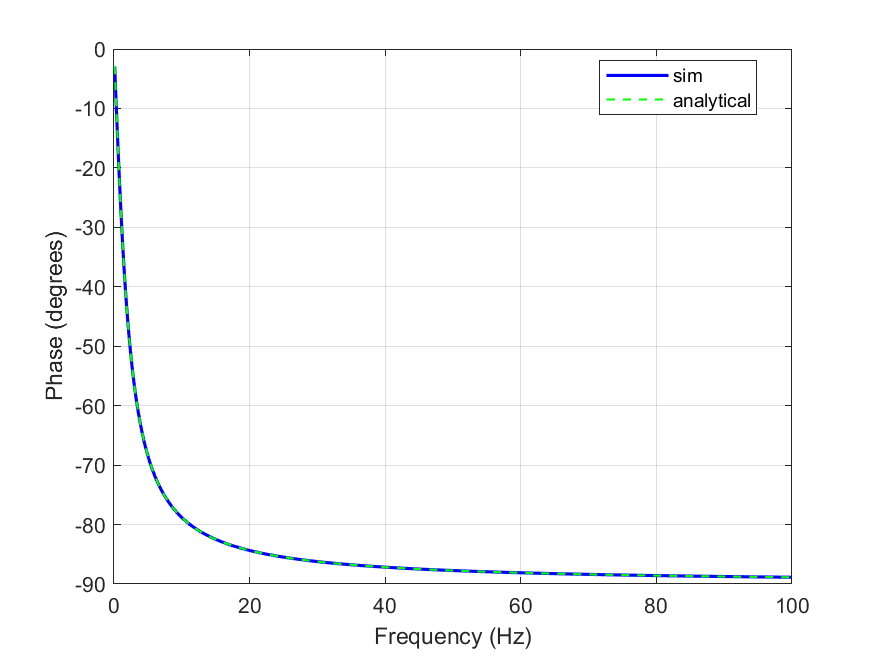
\includegraphics[width=0.8\textwidth]{freq_phase1.png}
  \caption{Сравнение - ФЧХ}
  \end{figure}
\newpage
\begin{figure}[ht]
    \centering
    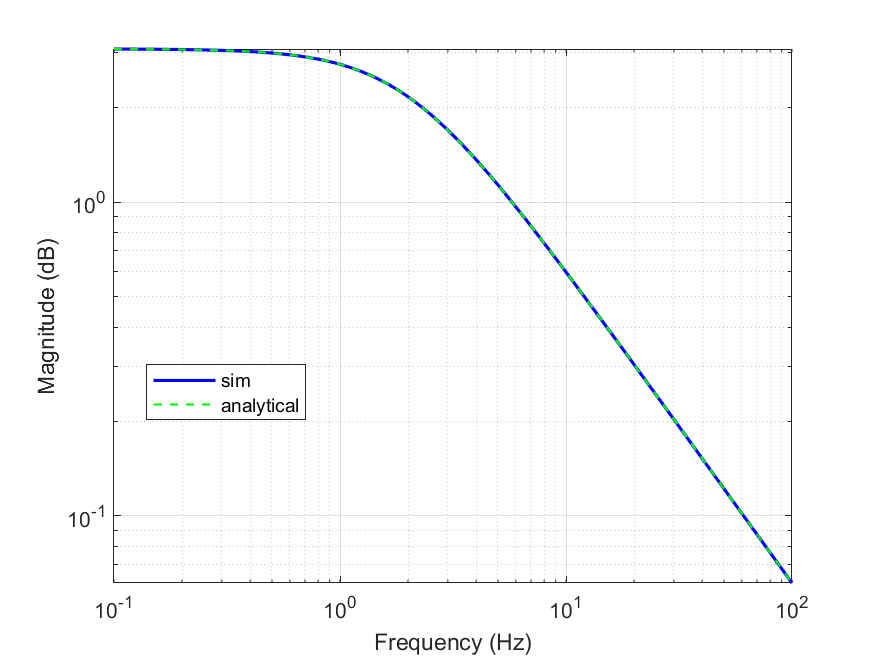
\includegraphics[width=0.8\textwidth]{lfreq_ampl1.png}
  \caption{Сравнение - ЛАЧХ}
  \end{figure}
  
  \begin{figure}[ht]
      \centering
      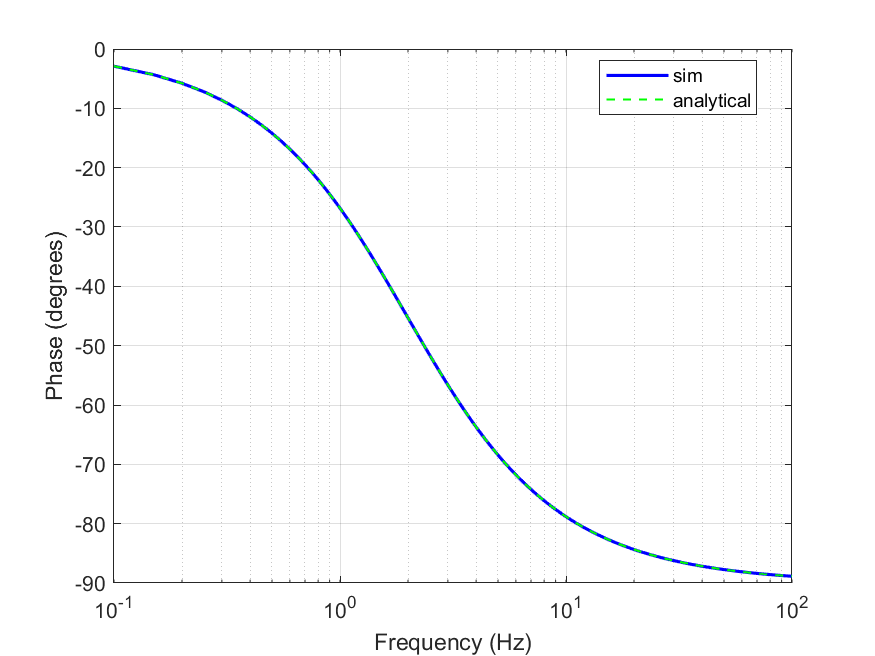
\includegraphics[width=0.8\textwidth]{lfreq_phase1.png}
    \caption{Сравнение - ЛФЧХ}
    \end{figure}

    % \begin{figure}[ht]
    %   \centering
    %   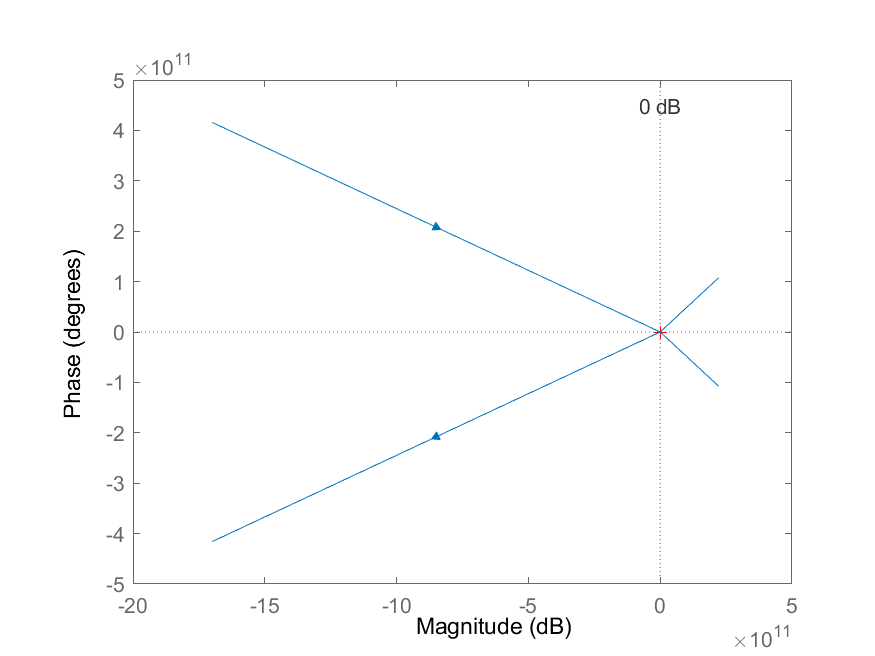
\includegraphics[width=0.8\textwidth]{nyquist1.png}
    % \caption{АФЧХ}
    % \end{figure}
\newpage

\endinput